\graphicspath{{./Figs/}}

\chapter{Results and Discussion} 

\section{Wind Tunnel Results}

\subsection{Aerodynamic Coefficient of Lift}

\subsection{Aerodynamic Coefficient of Drag}

\begin{figure}
    \centering
    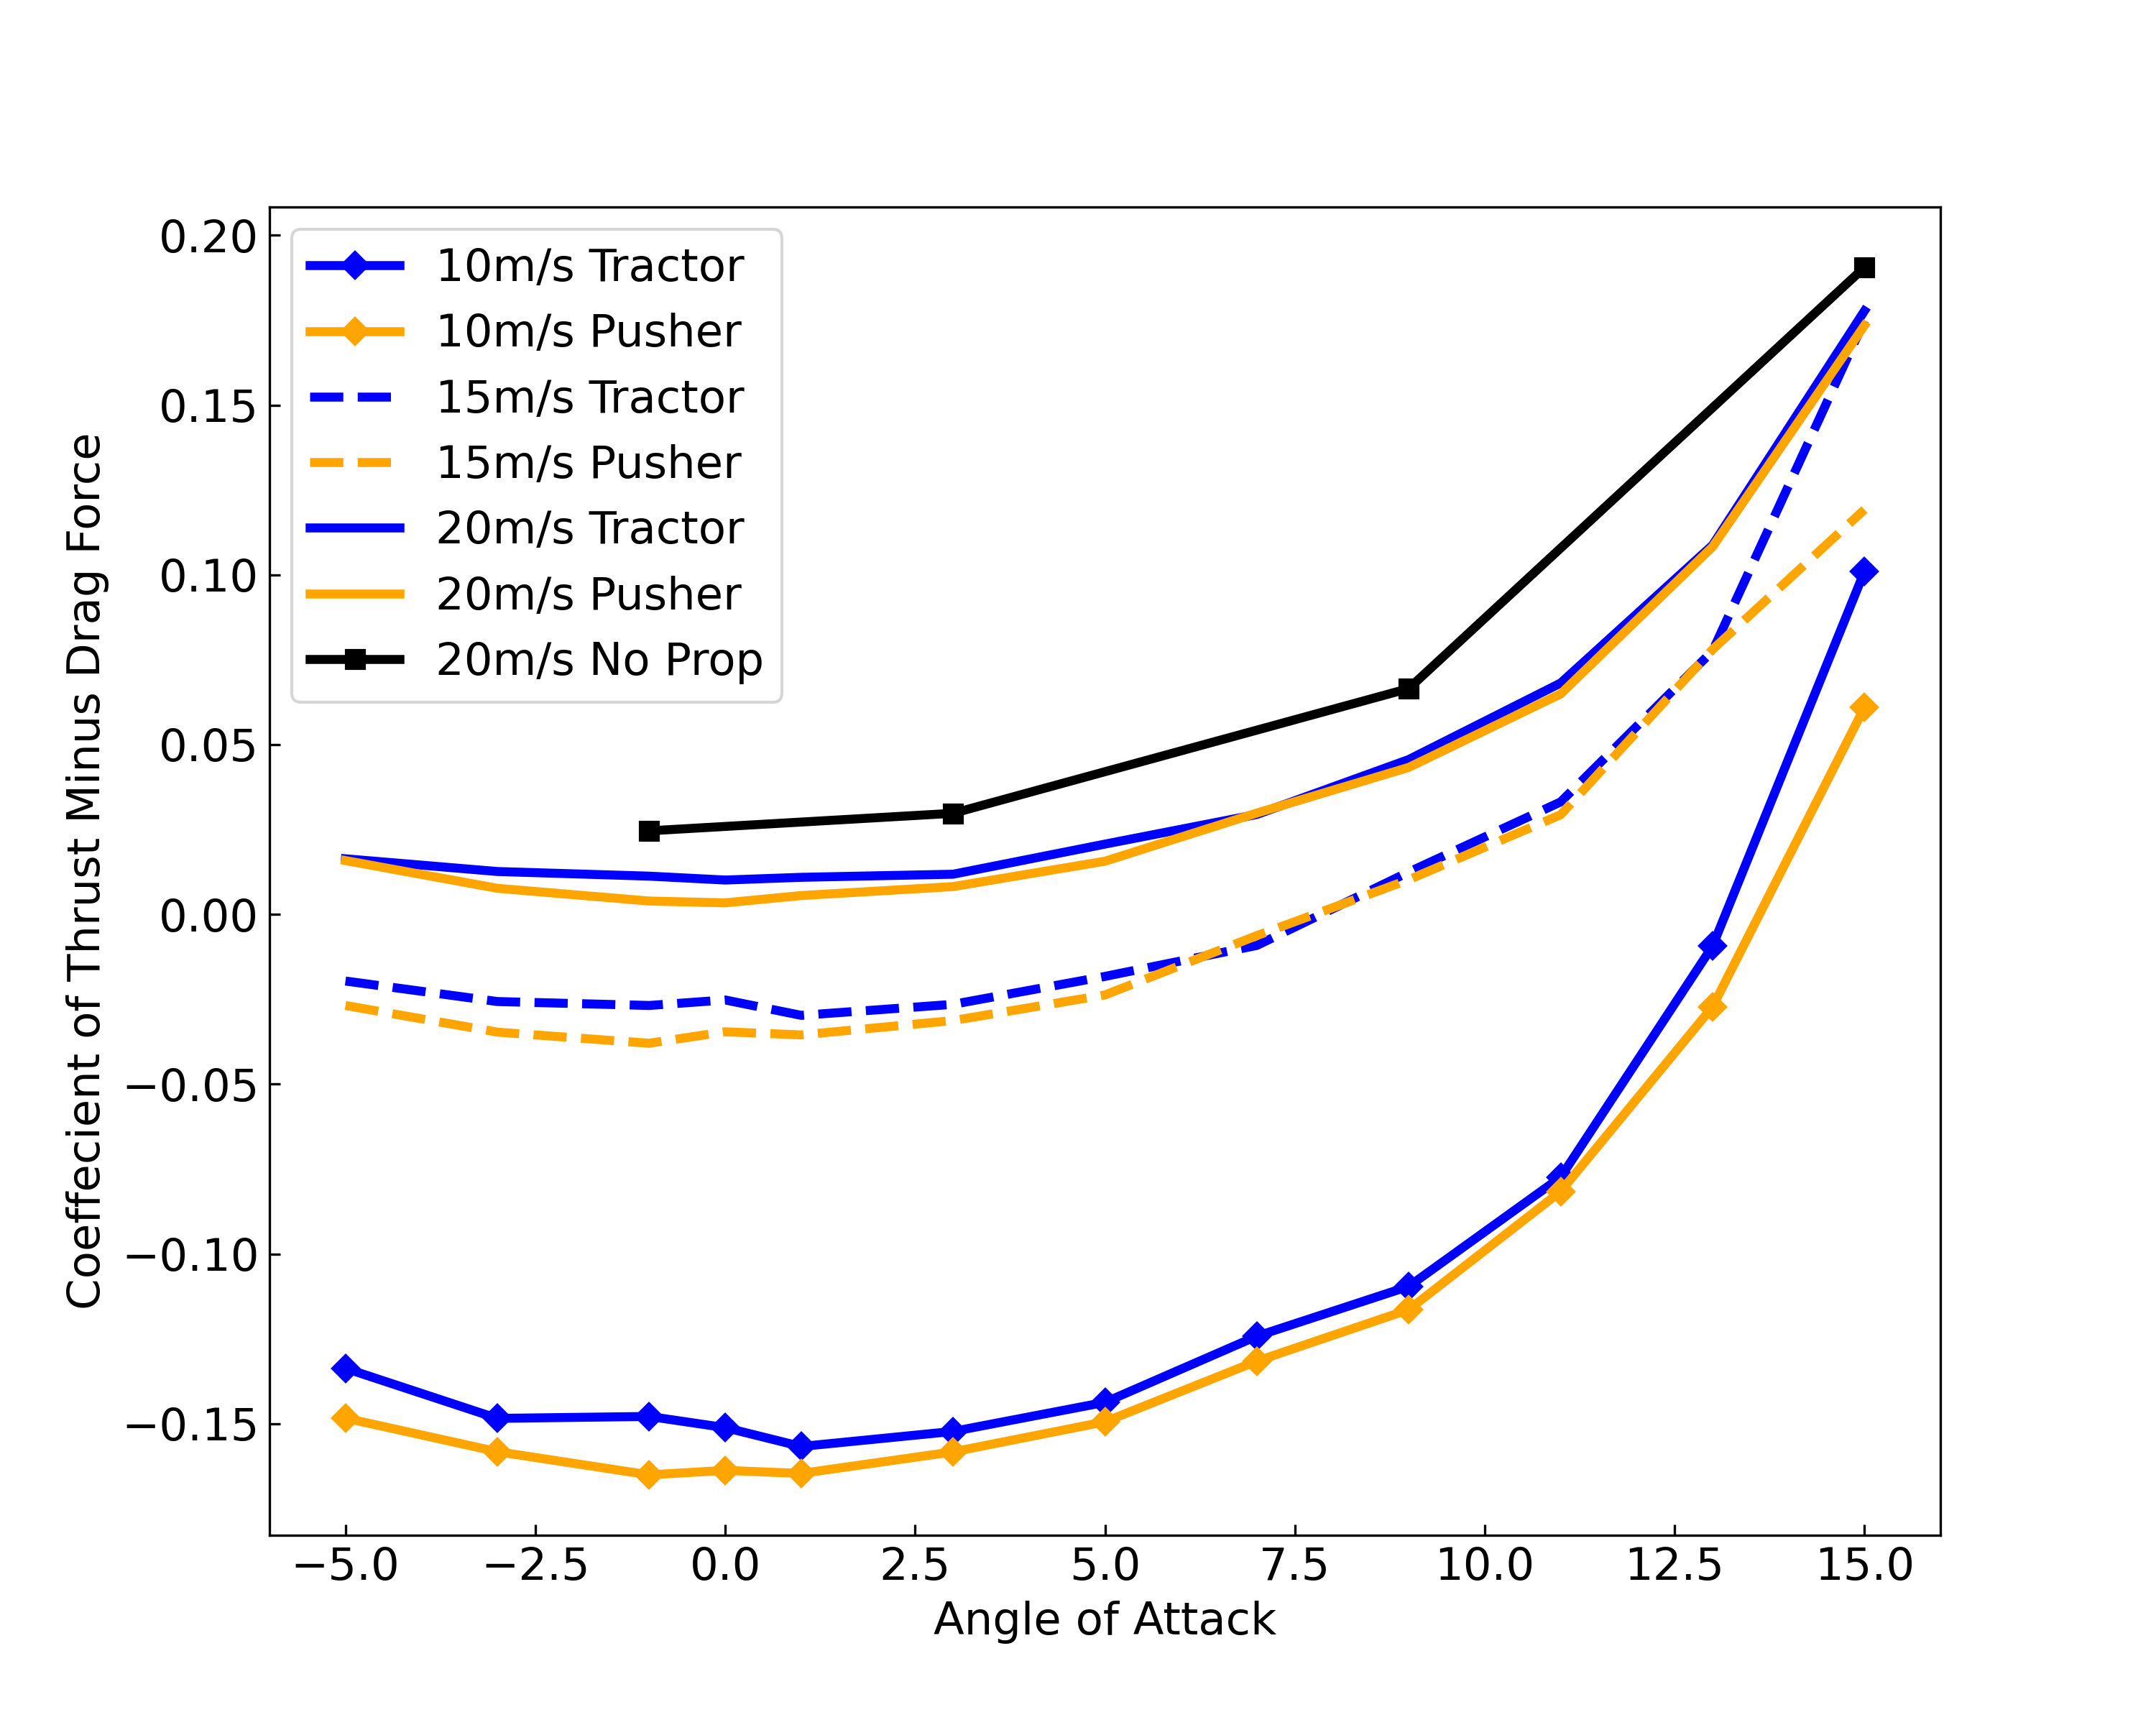
\includegraphics[scale = 0.1] {05_Results/Figs/Cd/110000RPM_Cd.png}
    \caption{Caption}
    \label{fig:Cd_11000RPM}
\end{figure}

\subsection{Moment Coefficient o}


\section{VAP Validation}

\subsection{Wing Validation}


\begin{figure}[H]
     \centering
     \begin{subfigure}[b]{0.45\textwidth}
         \centering
         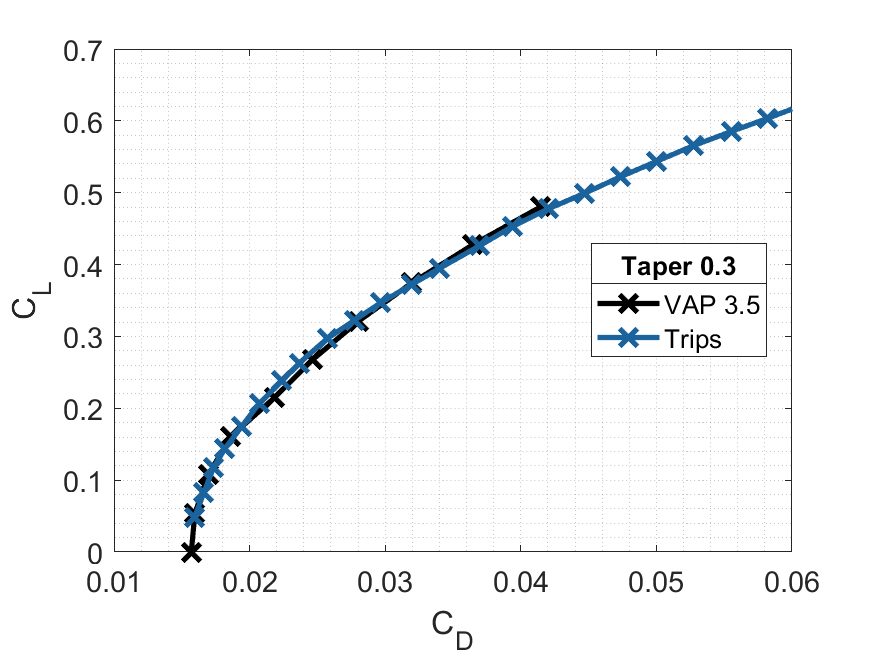
\includegraphics[width=\textwidth]{05_Results/Figs/VAP/genMAV/taper3a.png}

     \end{subfigure}
     \hfill
     \begin{subfigure}[b]{0.45\textwidth}
         \centering
         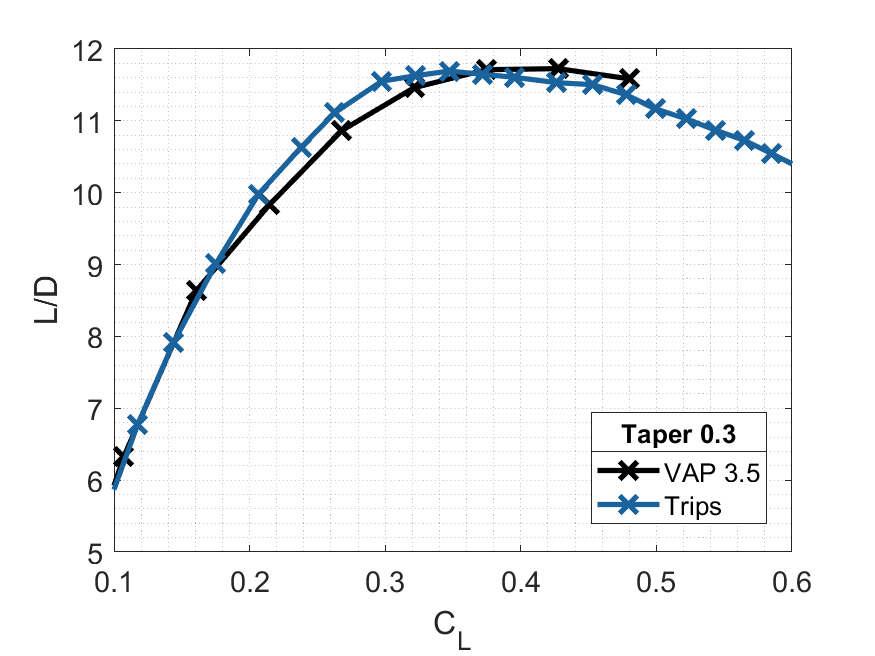
\includegraphics[width=\textwidth]{05_Results/Figs/VAP/genMAV/taper3b.png}
      
     \end{subfigure}
     \hfill

        
\end{figure}


\begin{figure}[H]
     \centering
     \begin{subfigure}[b]{0.45\textwidth}
         \centering
         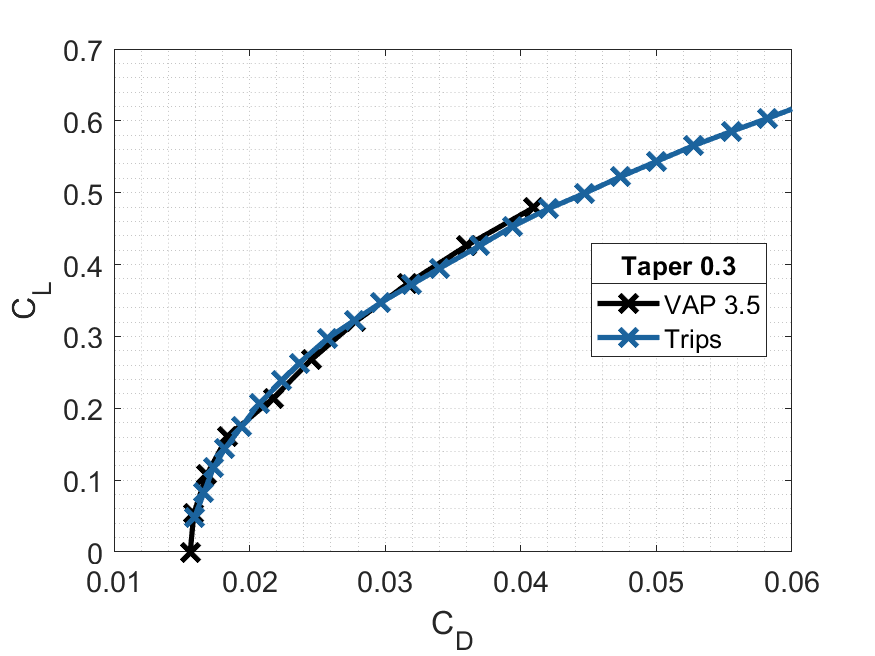
\includegraphics[width=\textwidth]{05_Results/Figs/VAP/genMAV/taper5a.png}

     \end{subfigure}
     \hfill
     \begin{subfigure}[b]{0.45\textwidth}
         \centering
         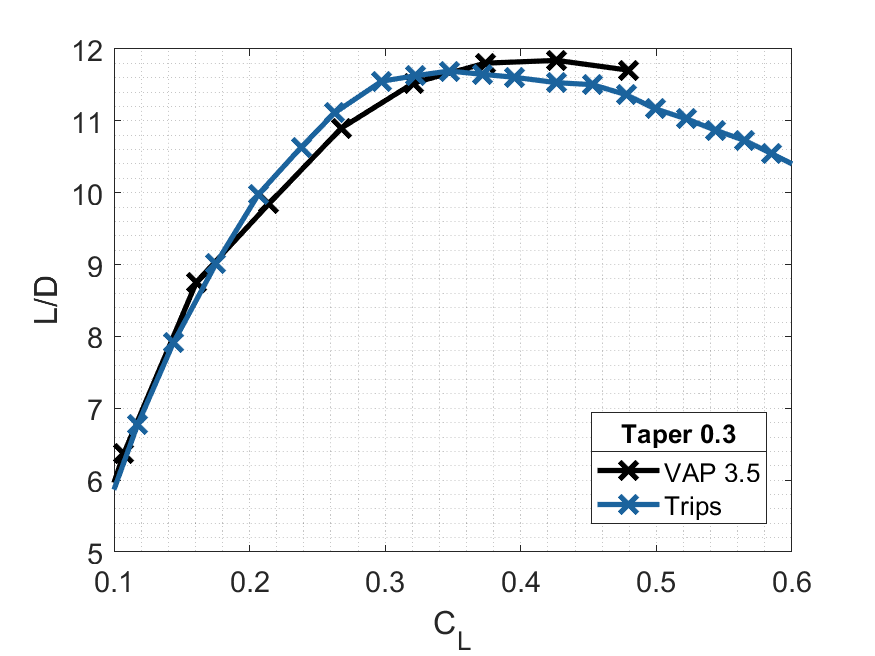
\includegraphics[width=\textwidth]{05_Results/Figs/VAP/genMAV/taper5b.png}
      
     \end{subfigure}
     \hfill

        
\end{figure}


\begin{figure}[H]
     \centering
     \begin{subfigure}[b]{0.45\textwidth}
         \centering
         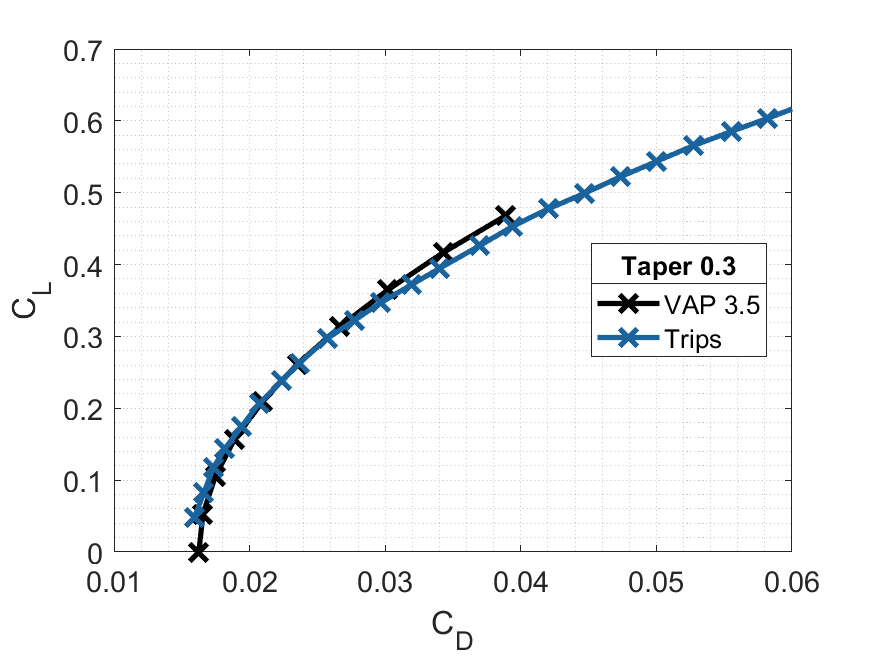
\includegraphics[width=\textwidth]{05_Results/Figs/VAP/genMAV/taper10a.png}

     \end{subfigure}
     \hfill
     \begin{subfigure}[b]{0.45\textwidth}
         \centering
         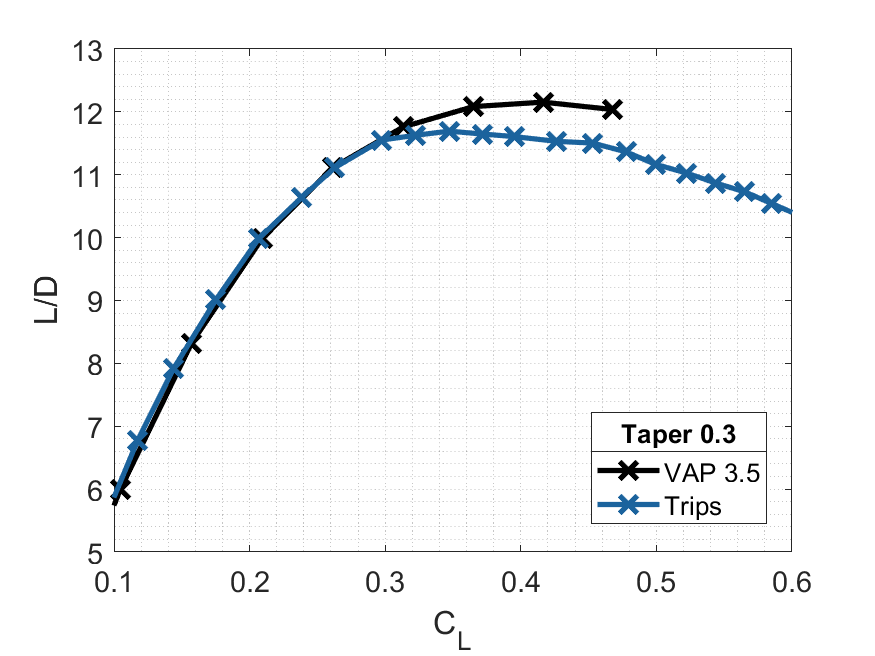
\includegraphics[width=\textwidth]{05_Results/Figs/VAP/genMAV/taper10b.png}
      
     \end{subfigure}
     \hfill

        
\end{figure}




\section{Discussion}